 \documentclass[12pt]{article}
\usepackage[a4paper, margin=.30in]{geometry}

\usepackage{array}
\usepackage{graphicx, subfig, wrapfig, fancyhdr, lastpage }
\newcommand\headerMe[2]{\noindent{}#1\hfill#2}
\usepackage[mathscr]{euscript}



\pagestyle{fancy}
\fancyhf{}

\rfoot{\em{Page \thepage \hspace{1pt} / \pageref{LastPage}}}
\begin{document}

\headerMe{Royaume du Maroc}{année scolaire \emph{2021-2022}}\\
\headerMe{Ministère de l'Éducation nationale, }{  Professeur :\emph{Zakaria Haouzan}}\\
\headerMe{du Préscolaire et des Sports}{Établissement : \emph{Lycée SKHOR qualifiant}}\\

\begin{center}
Devoir  N°2 \\
   Filière Tronc Commun Scientifique\\
Durée 2h00
\\
    \vspace{.2cm}
\hrulefill
\Large{Chimie 7pts}
\hrulefill\\

    %\emph{Les Trois parties sont indépendantes}
\end{center}
%end Headerss------------------------
 \section*{Partie 1 :Les pluies acides \dotfill (4pts) }
La principale cause des pluies acides est le rejet dans l'atmosphère de trioxyde de soufre $(SO_3)$ par les industries ou les voitures. En effet, le trioxyde de soufre SO3 réagit avec les gouttelettes d'eau de pluie et il se forme de l'acide sulfurique $H_2SO_4$, une des causes des pluies acides, responsables de la mort de certains arbre.

\begin{enumerate}
    \item Calculer la masse molaire moléculaire du trioxyde de soufre. \dotfill(1pt)
    \item On détecte dans l'aire d'une ville une quantité de matière de trioxyde de soufre égale à $3,20\mu mol$ par $m^3$ d'air. L'union européenne indique que les rejets de trioxyde de soufre ne doivent pas dépasser $300\mu g$ par $m^3$
d'aire.
        \begin{enumerate}
    \item Déterminer la masse de trioxyde de soufre dans la ville. \dotfill(1pt)
    \item L'aire de cette ville est-il considéré comme pollué? \dotfill(2pt)
        \end{enumerate}
\end{enumerate}
Données: $M(H) = 1 g/mol$ ; $M(O) = 16 g/mol$ ; $M(S) = 32,1 g/mol$.
\section*{Partie 2 :La quantité de matière du cholestérol\dotfill(3pts) }
Cholestérol $C_xH_{2x-8}O$ est une Substance lipide retrouvée dans le sang et de masse molaire est $M$=$386g/mol$. Le rapport normal de cette substance dans le sang compris entre $1,4g$ par litre et $2,2g$ par litre.
\begin{enumerate}
    \item Donner l'expression de masse molaire en fonction de x.\dotfill(1pt)
    \item Calculer x et déduire la formule brute du cholestérol.\dotfill(1pt)
    \item Le processus d'analyse sanguine a donné le résultat : le cholestérol est de $6,5mmol$ par litre de sang. Ce personne est-il en bonne santé ou malade?\dotfill(1pt)
\end{enumerate}
%__________________Chimie ______________________-
%%%%%%%+_+_+_+_+_+_+_+_+_Partie1

%_____________________________________PHYSIque Partie 22222____________________________________________________________________________
\begin{center}
    \vspace{1cm}
\hrulefill
\Large{Physique 13pts}
\hrulefill\\
    \emph{Les deux parties sont indépendantes}
\end{center}
%end Headerss------------------------
%_________________partie 2  : gravitation universelle :)
\section*{Partie 1 : La Mesure de l’intensité du courant éléctrique: \dotfill(7pts)}

%\begin{wrapfigure}[6]{r}{0.40\textwidth}
    %\vspace{-1cm}
%\begin{center}
    %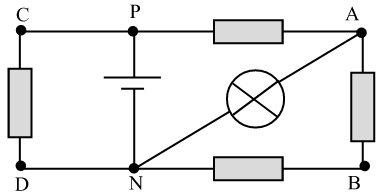
\includegraphics[width=0.36\textwidth]{./img/circuit_01.png}
%\end{center}
    %\end{wrapfigure}

Un courant continu a une intensité $I = 0,4 A$. 
\begin{enumerate}

    \item Calculer la quantité d'électricité Q débitée en 8 secondes.\dotfill(1pt)
    \item Déterminer le nombre d'électrons (n) traversant une section du conducteur pendant ce temps.\dotfill(1pt) 
    \item On désire mesurer un courant de 300mA à l'aide d'un ampèremètre dont le cadran comporte 100 divisions.Les calibres de l'ampèremètre sont les suivants: 5A; 500mA; 50mA. 
        \begin{enumerate}
            \item Comment doit-on brancher l'ampèremètre dans le circuit?\dotfill(1pt) 
            \item Quel calibre doit-on choisir. justifier la réponse. \dotfill(1pt)
            \item Sur quelle graduation se fixera l'aiguille de l'ampèremètre?\dotfill(1pt)
            \item Calculer l’incertitude absolue sur la mesure de l’intensité. Déduire l’incertitude relative. On donne:la classe de l’appareil est x = 1,5 .\dotfill(2pt)
\end{enumerate}
        \end{enumerate}
%\vspace{3cm}

\hrulefill\\

 \section*{Partie 2 :Le courant électrique continu \dotfill(6 pts)}
On considère le circuit de la figure 1: 

\begin{enumerate}
    \item Que peut-on dire des deux points A et B?\dotfill(1pt)
    \item Indiquer le sens des courants manquants
dans chaque branche du circuit. \dotfill(1pt)
                \item Pour mesurer l’intensité I, on utilise un ampèremètre à aiguille dont le calibre est fixé à 10 A et son aiguille indique la graduation 85. Calculer I.  \dotfill(1pt)
                \item En Déterminer la  relation entre I, $I_1$, $I_2$ et $I_3$; aussi Une relation entre $I_1$, $I_2$, et $I_4$; Une relation entre $I_3$, $I_4$, $I_5$ et $I_6$.\dotfill(2pt) 
    \item Sachant que $I_2 = 2 A$, $I_3 = 3 A$ et $I_6 = 1,5 A$, calculer les intensités manquantes.\dotfill(1pt)

\end{enumerate}
\begin{center}

    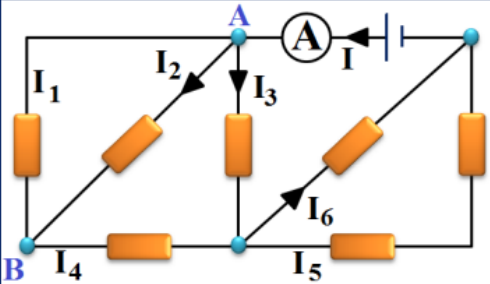
\includegraphics[width=0.36\textwidth]{./img/exo_00.png}
\end{center}


\end{document}
